\documentclass{beamer}
\mode<presentation>
\usepackage[T1]{fontenc}
\usepackage{tikz}
\usetikzlibrary {calc,graphs,graphs.standard,patterns.meta}
\usepackage[dvipsnames]{xcolor}
\usepackage{skak}
\usepackage{chessboard}
\usepackage{physics}
\tikzdeclarepattern{
name=mylines,
parameters={
\pgfkeysvalueof{/pgf/pattern keys/size},
\pgfkeysvalueof{/pgf/pattern keys/angle},
\pgfkeysvalueof{/pgf/pattern keys/line width},
},
bounding box={
(0,-0.5*\pgfkeysvalueof{/pgf/pattern keys/line width}) and
(\pgfkeysvalueof{/pgf/pattern keys/size},
0.5*\pgfkeysvalueof{/pgf/pattern keys/line width})},
tile size={(\pgfkeysvalueof{/pgf/pattern keys/size},
\pgfkeysvalueof{/pgf/pattern keys/size})},
tile transformation={rotate=\pgfkeysvalueof{/pgf/pattern keys/angle}},
defaults={
size/.initial=5pt,
angle/.initial=45,
line width/.initial=.4pt,
},
code={
\draw [line width=\pgfkeysvalueof{/pgf/pattern keys/line width}]
(0,0) -- (\pgfkeysvalueof{/pgf/pattern keys/size},0);
},
}
\title{Graphs and its Applications}
\author[dishajk]{Disha Kuzhively\\disha.jk@icts.res.in}
\institute{ICTS-TIFR}
\date[Palakkad]{1 April 2025}
\begin{document}
\begin{frame}
    \titlepage
\end{frame}
% \begin{frame}
% \frametitle{Outline}
% \tableofcontents[pausesections]
% \end{frame}
\section{Recap of Graphs}
\begin{frame}
    \frametitle{Recap of Graphs} 
    \begin{columns}[c]
      \begin{column}{0.4\textwidth}
    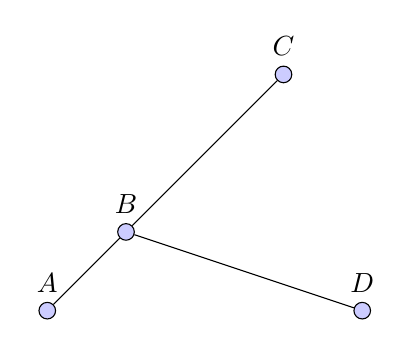
\begin{tikzpicture}
      \graph [
    nodes={
        circle,
        draw,
        fill=blue!20,      % Fills the circle with a color
        minimum size=6pt,  % Reduces the radius/size of the circle
        inner sep=0pt      % Removes internal padding so it stays small
    },
    empty nodes            % Clears the default text from inside the circles
]
{ 
    a[label=above:$A$] -- 
    b[at={(0,1)},label=above:$B$] -- 
    {
        c[at={(1,3)},label=above:$C$], 
        d[at={(2,1)},label=above:$D$]
    } 
};
    \end{tikzpicture}
          \end{column}
      \begin{column}{0.6\textwidth}
    \only<2->{
    \begin{itemize}
    \item $A, B, C, D$ are the \alert{vertices}.
    \item $AB, BC, BD$ are the \alert{edges}.
    \item The number of edges that start at a given vertex is called the \item{degree} of a vertex.
    \end{itemize}
    }
    \only<3->{
      \begin{block}{Question}
      What are the degrees of the vertices $A, B, C, D$?
      \end{block} 
    }
      \end{column}
    \end{columns}
\end{frame}
\section{Modeling Problems as Graphs}
\begin{frame}
\frametitle{Modeling Scenarios}
\only<1-2>{
  4 people, all friends with each other
  }
  \only<2>{
    \newline
    \centering
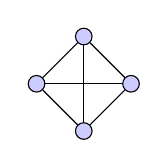
\begin{tikzpicture}
\graph [
    nodes={
        circle,
        draw,
        fill=blue!20,      % Fills the circle with a color
        minimum size=6pt,  % Reduces the radius/size of the circle
        inner sep=0pt      % Removes internal padding so it stays small
    },
    empty nodes            % Clears the default text from inside the circles
]{ subgraph K_n [--
, n=4, clockwise, radius=6mm] };
\end{tikzpicture}
}
\only<3-4>{
  4 computers, each connected to 2 others
  }
  \only<4>{
    \newline
            \centering
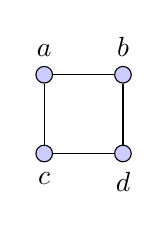
\begin{tikzpicture}
\graph [
    nodes={
        circle,
        draw,
        fill=blue!20,      % Fills the circle with a color
        minimum size=6pt,  % Reduces the radius/size of the circle
        inner sep=0pt      % Removes internal padding so it stays small
    },
    empty nodes,            % Clears the default text from inside the circles
    no placement
]
{ 
    a[label=above:$a$] -- { 
        b[at={(1,0)},label=above:$b$] -- {d[at={(1,-1)},label=below:$d$]}, 
        c[at={(0,-1)},label=below:$c$] -- d
    },
    % Connect the bottom row of nodes
    % b -- d
    
};
\end{tikzpicture}
}
\only<5-6>{
  a molecule of methane, $CH_4$, with 1 atom of carbon $(C)$ connected to 4 atoms of hydrogen $(H)$.
  }
\only<6>{
    \newline
    \centering
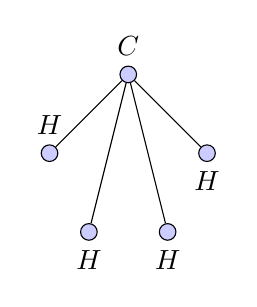
\begin{tikzpicture}
\graph [
    nodes={
        circle,
        draw,
        fill=blue!20,      % Fills the circle with a color
        minimum size=6pt,  % Reduces the radius/size of the circle
        inner sep=0pt      % Removes internal padding so it stays small
    },
    empty nodes,            % Clears the default text from inside the circles
    no placement
]
{ 
    a[at={(0,2)},label=above:$C$] -- { 
        b[at={(-1,1)},label=above:$H$], 
        c[at={(-1/2,0)},label=below:$H$],
        d[at={(1/2,0)},label=below:$H$], 
        e[at={(1,1)},label=below:$H$] 
    },    
};
\end{tikzpicture}
}
\end{frame}
\begin{frame}
  \frametitle{Modeling problems}
  \only<1>{
  Can we create graphs to describe situtations maths problems?
}
    \only<2>{
There are 5 computers connected with several cables to make a network. Each cable connects a pair of computers and every computer is connected to two other computers.
  }
  \only<3>{
    Several knights are situated on a 3 x 3 chessboard as shown in the Figure 1. Can they move, using the usual chess knight's move, to the position shown in Figure 2?

\setchessboard{
normalboard,
maxfield=c3,
setpieces={na1,nc1,Na3,Nc3},
showmover=false}
\chessboard

\setchessboard{
normalboard,
maxfield=c3,
setpieces={na1,Nc1,Na3,nc3},
showmover=false}
\chessboard
  }
\only<4>{
  A farmer has to take a tiger, a goat, and some melons across a river. Their boat has enough room for themself plus either the tiger, the goat, or the melons. If they take the melons with them, the tiger will eat the goat. If they takes the tiger across, the goat will eat the melons. Only when the farmer is present are the goat and the melons safe from their enemies. All the same, the farmer successfully carries the tiger, the goat, and the melons across the river. How?
}
\only<5>{
  Can a knight travel around this board, pass through each square exactly once, and end on the same square it starts on?
\chessboard[pgfstyle=cross,
maxfield=d4,
color=red,
padding=-0.2em,
pgfstyle=cross,
markfields={a1,a4,d1,d4}
]
}
\end{frame}
\section{Problems}
\begin{frame}
  \frametitle{Vertices and Edges}
\only<1>{
  A couple invites 10 people to a house party. The hosts shake hands with everyone but each other. The guests shake hands with everyone else in the party. How many handshakes took place?
}
\only<2>{
  IRTC has 9 computers. They want to link them into a network so that every computer would be connected with exactly 4 computers by network cables.
  \begin{enumerate}
\item How many cables will they need? Can you draw such a configuration?
\item They decided to connect every computer with exactly 5 other computers. Is this a possible configuration?
  \end{enumerate}
}
\only<3>{
  In Kottayam, there are 9 constituencies; some are connected by roads, and others are not. (A road connects a pair of constituencies with each other.) Is it possible that each of the constituencies is connected to exactly 3 other constituencies?
}
\end{frame}
\section{Handshake Theorem}
\begin{frame}
  Sum of the degrees of all vertices should be an even = 2 times number of edges.
  \uncover<2->{
  \begin{block}{Handshake Theorem}  
  For any graph the number of vertices with an odd degree must be even.
  \end{block}
  }
\end{frame}
\begin{frame}
  \begin{tikzpicture}
    \coordinate (A) at (0,0);
    \coordinate (B) at (6,0);
    \coordinate (C) at (60:6);
    \draw (A) -- (B) -- (C) -- cycle;
    \uncover<2->{
    \filldraw [SkyBlue] (A) circle [radius=2pt];
    \filldraw [Orange] (B) circle [radius=2pt];
    \filldraw [darkgray] (C) circle [radius=2pt];
    }
    \uncover<3->{
      \foreach \i in {1,...,4}{
        \coordinate (ab\i) at ($ (A)!{.2*\i}!(B) $);
      }
    \filldraw [SkyBlue] (ab1) circle [radius=2pt];
    \filldraw [Orange] (ab2) circle [radius=2pt];
    \filldraw [SkyBlue] (ab3) circle [radius=2pt];
    \filldraw [SkyBlue] (ab4) circle [radius=2pt];
    }
    \uncover<4->{
      \foreach \i in {1,...,4}{
        \coordinate (ac\i) at ($ (A)!{.2*\i}!(C) $);
        \coordinate (bc\i) at ($ (B)!{.2*\i}!(C) $);
      }
    \filldraw [SkyBlue] (ac1) circle [radius=2pt];
    \filldraw [darkgray] (ac2) circle [radius=2pt];
    \filldraw [darkgray] (ac3) circle [radius=2pt];
    \filldraw [SkyBlue] (ac4) circle [radius=2pt];

    \filldraw [Orange] (bc1) circle [radius=2pt];
    \filldraw [darkgray] (bc2) circle [radius=2pt];
    \filldraw [Orange] (bc3) circle [radius=2pt];
    \filldraw [darkgray] (bc4) circle [radius=2pt];
    }
    \uncover<5->{
      \foreach \i in {1,...,4}{
        \pgfmathsetmacro{\j}{int(5 - \i)}
        \draw (ac\i) -- (bc\i);
        \draw (ab\i) -- (ac\i);
        \draw (ab\i) -- (bc\j);
      }
    }
    \uncover<6->{
    \coordinate (r1) at ($ (ac1)!.25!(bc1) $);
    \filldraw [Orange] (r1) circle [radius=2pt];

    \coordinate (r2) at ($ (ac1)!.5!(bc1) $);
    \filldraw [SkyBlue] (r2) circle [radius=2pt];

    \coordinate (r3) at ($ (ac1)!.75!(bc1) $);
    \filldraw [darkgray] (r3) circle [radius=2pt];

    \coordinate (r4) at ($ (ab1)!.5!(bc4) $);
    \filldraw [Orange] (r4) circle [radius=2pt];
    
    \coordinate (r5) at ($ (ab1)!.75!(bc4) $);
    \filldraw [Orange] (r5) circle [radius=2pt];

    \coordinate (r6) at ($ (ab4)!.5!(ac4) $);
    \filldraw [SkyBlue] (r6) circle [radius=2pt];
    }
    \uncover<7->{
    \draw[pattern={mylines[size= 5pt,line width=.8pt,angle=40]}, pattern color=red] (ac1) -- (r1) -- (ac2) -- cycle;
    \draw[pattern={mylines[size= 5pt,line width=.8pt,angle=40]}, pattern color=red] (ac3) -- (ac4) -- (r5) -- cycle;
    \draw[pattern={mylines[size= 5pt,line width=.8pt,angle=40]}, pattern color=red] (bc2) -- (bc3) -- (r6) -- cycle;
    \draw[pattern={mylines[size= 5pt,line width=.8pt,angle=40]}, pattern color=red] (ac4) -- (bc4) -- (r5) -- cycle;
    \draw[pattern={mylines[size= 5pt,line width=.8pt,angle=40]}, pattern color=red] (r3) -- (bc1) -- (ab4) -- cycle;
    }
        \uncover<10->{
      \coordinate (c1) at ($($(ac1)!.5!(r1)$)!{1/(2*sqrt(3))}!(ac2)$);
      \coordinate (c2) at ($($(ab1)!.5!(r1)$)!{1/(2*sqrt(3))}!(ac1)$);
      \coordinate (c3) at ($($(ab1)!.5!(ab2)$)!{1/(2*sqrt(3))}!(r1)$);
      \draw[ultra thick] (c1) -- (c2) -- (c3) -- ++(-90:1);
      \coordinate (c4) at ($($(ac3)!.5!(r5)$)!{1/(2*sqrt(3))}!(ac4)$);
      \coordinate (c5) at ($($(r5)!.5!(bc4)$)!{1/(2*sqrt(3))}!(ac4)$);
      \draw[ultra thick] (c4) -- (c5);
      \coordinate (c6) at ($($(r6)!.5!(bc3)$)!{1/(2*sqrt(3))}!(bc2)$);
      \coordinate (c7) at ($($(r6)!.5!(bc3)$)!{1/(2*sqrt(3))}!(r5)$);
      \coordinate (c8) at ($($(r1)!.5!(r2)$)!{1/(2*sqrt(3))}!(ab2)$);
      \coordinate (c9) at ($($(ab2)!.5!(r2)$)!{1/(2*sqrt(3))}!(ab3)$);
      \draw[ultra thick] (c6) -- (c7) -- (c8) -- (c9) --++(-90:1);
      \coordinate (c10) at ($($(bc1)!.5!(r3)$)!{1/(2*sqrt(3))}!(ab4)$);
      \draw[ultra thick] (c10) --++(-30:{sqrt(3)/2}) --++(-90:1);
    }
\end{tikzpicture}
\only<8-9>{
  \newline
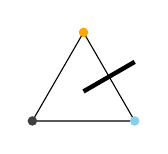
\begin{tikzpicture}[scale=0.75]
\draw (-30:1) -- (90:1) -- (210:1) --cycle;
\draw[ultra thick] (0:0) -- (30:1);
\filldraw [SkyBlue] (-30:1) circle [radius=2pt];
\filldraw [Orange] (90:1) circle [radius=2pt];
\filldraw [darkgray] (210:1) circle [radius=2pt];
\end{tikzpicture}
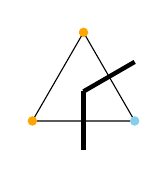
\begin{tikzpicture}[scale=0.75]
\draw (-30:1) -- (90:1) -- (210:1) --cycle;
\draw[ultra thick] (0:0) -- (-90:1);
\draw[ultra thick] (0:0) -- (30:1);
% \draw[ultra thick] (0:0) -- (150:1);
\filldraw [SkyBlue] (-30:1) circle [radius=2pt];
\filldraw [Orange] (90:1) circle [radius=2pt];
\filldraw [Orange] (210:1) circle [radius=2pt];
\end{tikzpicture}}
\only<9>{
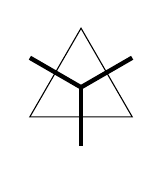
\begin{tikzpicture}[scale=0.75]
\draw (-30:1) -- (90:1) -- (210:1) --cycle;
\draw[ultra thick] (0:0) -- (-90:1);
\draw[ultra thick] (0:0) -- (30:1);
\draw[ultra thick] (0:0) -- (150:1);
\end{tikzpicture}}
\end{frame}
\begin{frame}

\begin{tikzpicture}[scale=0.75]
    \coordinate (A) at (0,0);
    \coordinate (B) at (6,0);
    \coordinate (C) at (3,4);
    \coordinate (ab1) at ($ (A)!.25!(B) $);
    \coordinate (ab2) at ($ (A)!.55!(B) $);
    \coordinate (ab3) at ($ (A)!.85!(B) $);
    \filldraw [SkyBlue] (A) circle [radius=2pt];
    \filldraw [Orange] (B) circle [radius=2pt];
    \filldraw [darkgray] (C) circle [radius=2pt];

    \draw (A) -- (B) -- (C) -- cycle;
    \filldraw [SkyBlue] (ab1) circle [radius=2pt];
    \filldraw [Orange] (ab2) circle [radius=2pt];
    \filldraw [SkyBlue] (ab3) circle [radius=2pt];

    \coordinate (ac1) at ($ (A)!.25!(C) $);
    \coordinate (ac2) at ($ (A)!.55!(C) $);
    \coordinate (ac3) at ($ (A)!.85!(C) $);

    \filldraw [SkyBlue] (ac1) circle [radius=2pt];
    \filldraw [darkgray] (ac2) circle [radius=2pt];
    \filldraw [darkgray] (ac3) circle [radius=2pt];

    \coordinate (bc1) at ($ (B)!.25!(C) $);
    \coordinate (bc2) at ($ (B)!.55!(C) $);
    \coordinate (bc3) at ($ (B)!.85!(C) $);

    \filldraw [Orange] (bc1) circle [radius=2pt];
    \filldraw [darkgray] (bc2) circle [radius=2pt];
    \filldraw [darkgray] (bc3) circle [radius=2pt];

    \coordinate (r1) at ($ (ac1)!.25!(bc1) $);
    \draw (r1) circle [radius=2pt];
    \filldraw [Orange] (r1) circle [radius=2pt];

    \coordinate (r2) at ($ (ac1)!.45!(bc1) $);
    \draw (r2) circle [radius=2pt];
    \filldraw [SkyBlue] (r2) circle [radius=2pt];

    \coordinate (r3) at ($ (ac1)!.8!(bc1) $);
    \draw (r3) circle [radius=2pt];
    \filldraw [darkgray] (r3) circle [radius=2pt];

    \coordinate (r4) at ($ (ac2)!rnd!(bc2) $);
    \draw (r4) circle [radius=2pt];
    \filldraw [Orange] (r4) circle [radius=2pt];

    \draw (ac1) -- (bc1);
    \draw (ac2) -- (bc2);
    \draw (ac3) -- (bc3);
    \draw (ac1) -- (ab1) -- (r1) -- (ab2) -- (r2) -- (ab3) -- (r3) -- (B);
    \draw (ac2) -- (r1) -- (r4) -- (r2) -- (bc2) -- (r3);
    \draw (ac3) -- (r4) -- (bc3);

    \draw[pattern={mylines[size= 5pt,line width=.8pt,angle=40]},
pattern color=red] (ab3) -- (r3) -- (B) -- cycle;
    \draw[pattern={mylines[size= 5pt,line width=.8pt,angle=40]},
pattern color=red] (ac1) -- (r1) -- (ac2) -- cycle;

    \draw[pattern={mylines[size= 5pt,line width=.8pt,angle=40]},
pattern color=red] (r2) -- (r4) -- (bc2) -- cycle;
\end{tikzpicture}
\only<2->{
  \begin{block}{Sperner Coloring}
    \begin{enumerate}
    \item Each of the three vertices $A, B,$ and $C$ of the initial triangle has a distinct color.
    \item The vertices that lie along any edge of triangle ABC have only two colors, the two colors at the endpoints of the edge. For example, each vertex on AC must have the same color as A or C.
    \end{enumerate}
  \end{block}
  \begin{block}{Sperner's Lemma}
    Sperner coloring of every triangulation has odd number of multicolored triangles
  \end{block}
}
\end{frame}
\begin{frame}
  \frametitle{Coloring}
  In a group of 6 students, every pair of students are either friends or enemies. Prove that it is possible to choose 3 of these students so that they are either all friends or all enemies.
\end{frame}
\begin{frame}
  \frametitle{More Problems}
  \only<1>{
  The number of vertices with an odd degree must be even.\\
  Graphs with odd numbers of odd degree vertices are impossible. Is the opposite equally true?

    Can you draw a graph that has 5 vertices, in which the degrees of these vertices are 4, 4, 4, 2, and 2? Either draw such a graph or explain why it is impossible.
  }
  \only<2>{
The 8 heads of state of SAARC got together for a conference. According to a reporter, each of the heads of Afghanistan, Bangladesh, and Bhutan shook hands with 6 heads of state each, each of the heads of India, Maldives, and Nepal with 4, and each of the heads of Pakistan, and Sri Lanka with 1. Is the reporter correct?}
\only<3>{
  It is known that 3 edges meet at every vertex of a polyhedron. 
  Is it possible for this polyhedron to have exactly 9 vertices?
}
\only<4>{
   It is known that in a certain company, each employee has exactly 3 friends among the co-workers. 
  Is it possible that this company has exactly 9 employees?
}
\end{frame}
\section{References}
\begin{frame}
  \nocite{vpunit}
\nocite{Burago}
  \nocite{Fomin}
\bibliographystyle{ieeetr}
\bibliography{graphsApplications}
\end{frame}
\end{document}
  


  
 

